\setbackground
{
	\centering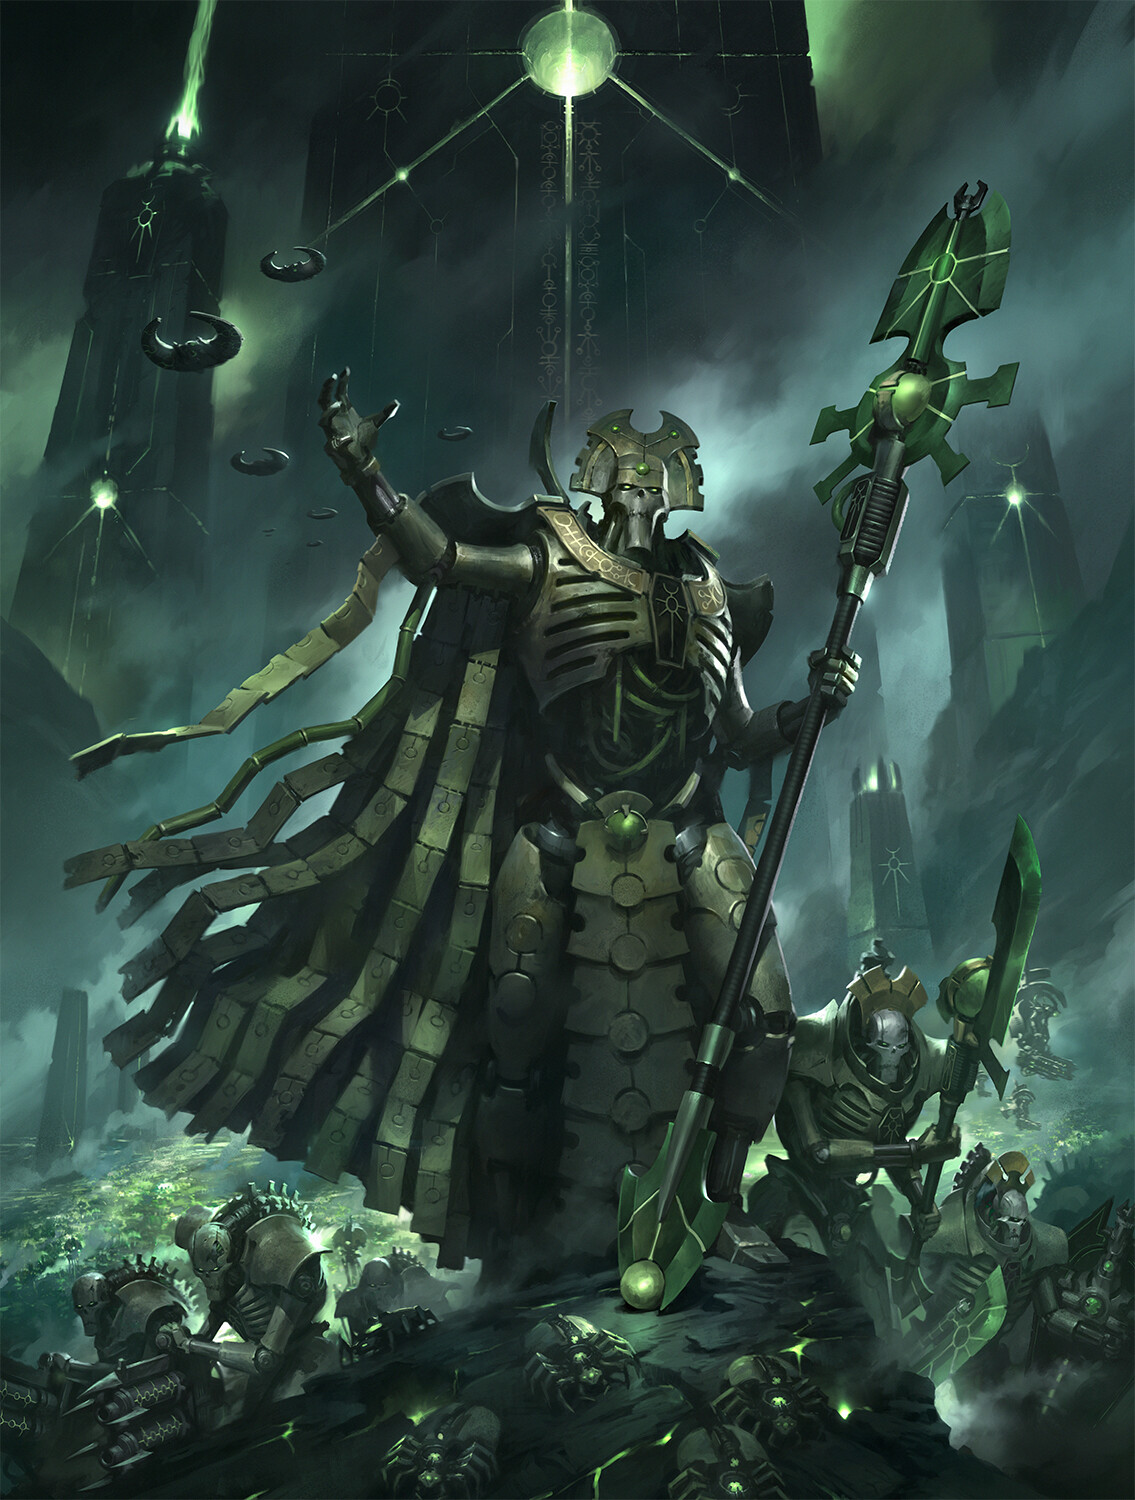
\includegraphics[height=530pt, width=400pt]{hq_art.jpg}
	\subsection[Lords of War]{\texorpdfstring{\centering\Huge Lords of War}{Lords of War}}
	
	\centerline{\begin{minipage}{400pt}
			\centering
			The silver prince nodded, and continued. ‘So, here is the lesson.’ 
			
			He extended his arm towards the far dust cloud, as if he were about to implore the oncoming Titans, still ten leagues or more away, with rhetoric. And he said one word: ‘Patience.’ 
			
			There was the tiniest, most insignificant little click. And in the same instant, the largest of the three walkers detonated, its central reactors struck dead-on by a sliver of metal moving faster than light itself. 
			
			\vspace*{1em}
			\raggedleft Djoseras
	\end{minipage}}
}

\newpage
\clearbackground
\subsubsection[Æonic Orb]{}
\fbox{\begin{imgminipage}{marble.jpg}[t][0.90\textheight]{0.2\textwidth}
		\color{white}
		\centering {\large LORDS OF WAR}
		
		\raggedright \small
		\color{black}
\end{imgminipage}}
\hspace{0.5em}
\begin{minipage}[t]{0.72\textwidth}
	{\large \textbf{Æonic Orb \dotfill X Points}}
	\begin{NiceTabular}{m{145 pt} *{2}{c} | *{3}{c} | c | c }
		& & & \cellgray{3}{Armour} & & & & \cellgray{1}{Transport} \\
		& M & BS & \cellgray{1}{Front} & \cellgray{1}{Side} & \cellgray{1}{Rear} & HP & \cellgray{1}{Capacity} \\
		\hline
		Æonic Orb & 12 & 5 & \cellgray{1}{14} & \cellgray{1}{14} & \cellgray{1}{14} & 18 &\cellgray{1}{—} \\
	\end{NiceTabular}
	\small
	\begin{minipage}[t]{0.5\textwidth}
		\begin{flushleft}
			\vspace*{2em}
			\textbf{Unit Composition}
			\begin{itemize}
				\item 1 Æonic Orb
			\end{itemize}
			
			\textbf{Wargear}
			\begin{itemize}
				\item \quickref{Quantum Shielding}
				\item \quickref{Quantum Shielding Matrix}
				\item Star Cage
			\end{itemize}
		\end{flushleft}
	\end{minipage}
	\begin{minipage}[t]{0.5\textwidth}
		\begin{flushleft}
			\vspace*{2em}
			\textbf{Unit Type}
			\begin{itemize}
				\item Super-Heavy Vehicle (\quickref{Living Metal}, Skimmer)
			\end{itemize}
			
			\textbf{Special Rules}
			\begin{itemize}
				\item Advanced Living Metal
				\item \quickref{Awakening Protocols} (Platinum)
				\item Catastrophic Destruction
				\item Power of the Machine Spirit
			\end{itemize}
		\end{flushleft}
	\end{minipage}
	
	\vspace*{2em}
	\textbf{Unit Rules}
	
	\textit{Advanced Living Metal:} This model's It Will Not Die level is increased to (1+).
	
	\vspace*{2em}
	\textbf{Weapons}
	
	\begin{tabular}{L{90 pt} c C{40pt} *{2}{c} >{\raggedright\arraybackslash}p{130pt}}
		& Range & Type & S & AP & Abilities \\
		\hline
		\quickref{Star Cage} & & & & & \\
		— Solar Burst & 72" & Destroyer 1 & 10 & 1 & Apocalyptic Blast, Blind, Ignores Cover, Lingering Death \\
		— Solar Flare & 180" & Destroyer 1 & 14 & 1 & Blind, Ignores Cover, \quickref{Path of Annihilation} (4)\\
	\end{tabular}
\end{minipage}



\newpage
\subsubsection[Doomsday Monolith]{}


\newpage
\subsubsection[Gauss Pylon]{}
% TODO: Decide here or forts


\newpage
\subsubsection[Sentry Pylon]{}
% TODO: Decide here or forts


\newpage
\subsubsection[Obelisk]{}


\newpage
\subsubsection[Seraptek Heavy Construct]{}
\fbox{\begin{imgminipage}{marble.jpg}[t][0.90\textheight]{0.2\textwidth}
		\color{bronze}
		\centering {\large Lords of War}
		
		\raggedright
		At the heart of many Necron tomb complexes, sleeping Seraptek Heavy Constructs await the footfall of intruders. These brutal war engines were designed by ancient Cryptek conclaves to protect each world’s master program, and this they do with merciless efficiency. Generators thrumming, the huge constructs advance with frightening speed, their optic lenses glowing as they pick out their targets. Massive cannons swivel in gimbal housings, crackling with destructive energies before unleashing pinpoint salvos to annihilate the interlopers. Should foes stray too close, the tomb guardians lash out with impaling forelimbs, their energy-sheathed tips rending metal, flesh and bone alike at a molecular level.
		
		As the legions of the Necron dynasties march out into the stars in ever-greater numbers, many Necron Overlords have summoned their Seraptek constructs to join their ranks, replacing their timeless vigils with front-line battlefield duties. In this capacity, Seraptek Heavy Constructs have proven mighty engines of conquest, more than capable of meeting an Imperial Knight or Ork Stompa head-on and emerging victorious.
		\raggedright \small
		\color{black}
\end{imgminipage}}
\hspace{0.5em}
\begin{minipage}[t]{0.72\textwidth}
	{\large \textbf{Seraptek Heavy Construct \dotfill X Points}}
	\begin{NiceTabular}{m{110 pt} *{4}{c} | *{3}{c} | c c c }
		& & & & & \cellgray{3}{Armour} & & & & & \\
		& M & WS & BS & S & \cellgray{1}{Front} & \cellgray{1}{Side} & \cellgray{1}{Rear} & I & A & HP \\
		\hline
		Seraptek Heavy Construct & 12 & 4 & 4 & 8 & \cellgray{1}{12} & \cellgray{1}{12} & \cellgray{1}{12} & 2 & 6 & 8 \\
	\end{NiceTabular}
	\small
	\begin{minipage}[t]{0.5\textwidth}
		\begin{flushleft}
			\vspace*{2em}
			\textbf{Unit Composition}
			\begin{itemize}
				\item 1 Seraptek Heavy Construct
			\end{itemize}
			
			\textbf{Wargear}
			\begin{itemize}
				\item Two Sponson Mounted \quickref{Sigularity Cannons}
			\end{itemize}
		\end{flushleft}
	\end{minipage}
	\begin{minipage}[t]{0.5\textwidth}
		\begin{flushleft}
			\vspace*{2em}
			\textbf{Unit Type}
			\begin{itemize}
				\item Vehicle (\quickref{Living Metal}, Knight)
			\end{itemize}
			
			\textbf{Special Rules}
			\begin{itemize}
				\item \quickref{Awakening Protocols} (Gold)
				\item Catastrophic Explosion
				\item Containment Field
				\item Night Vision
				\item \quickref{Quantum Shielding}
				\item \quickref{Tomb Guardians}
			\end{itemize}
		\end{flushleft}
	\end{minipage}
	
	\vspace*{2em}
	\textbf{Weapons}
	
	\begin{tabular}{L{90 pt} c C{40pt} *{2}{c} >{\raggedright\arraybackslash}p{130pt}}
		& Range & Type & S & AP & Abilities \\
		\hline
		\quickref{Singularity Cannon} & 36" & Heavy 1 & 8 & 2 & Large Blast, Haywire, Concussive (1), Perfect Singularity  \\
		\quickref{Synaptic Obliterator} & 72" & Destroyer 2 & 10 & 1 & Blast, Pinning \\
		\quickref{Transdimensional Projector} & 30" & Heavy 1 & 6 & 4 & Large Blast, \quickref{Exile Ray} (6+) \\
	\end{tabular}
	
	\vspace*{2em}
	\textbf{Unit Rules}
	
	\textit{Containment Field}: The Seraptek Heavy Construct has a 5+ Invulnerable Save. 
	
	\vspace*{2em}
	\textbf{Options}
	\begin{itemize}
		\item The Seraptekh Heavy Construct may exchange any \quickref{Singularity Cannon} for:
		\begin{itemize}
			\item \quickref{Synaptic Obliterator} and a \quickref{Transdimensional Projector} \dotfill +X points
		\end{itemize}
		\item The Seraptekh Heavy Construct may take:
		\begin{itemize}
			\item \quickref{Quantum Shielding Matrix} \dotfill +5 points
		\end{itemize} 
	\end{itemize}
\end{minipage}



\newpage
\subsubsection[Tesseract Vault]{}
\fbox{\begin{imgminipage}{marble.jpg}[t][0.90\textheight]{0.2\textwidth}
		\color{white}
		\centering {\large LORDS OF WAR}
		
		\raggedright \small
		\color{black}
\end{imgminipage}}
\hspace{0.5em}
\begin{minipage}[t]{0.72\textwidth}
	{\large \textbf{Tesseract Vault \dotfill X Points}}
	\begin{NiceTabular}{m{145 pt} *{2}{c} | *{3}{c} | c | c }
		& & & \cellgray{3}{Armour} & & & & \cellgray{1}{Transport} \\
		& M & BS & \cellgray{1}{Front} & \cellgray{1}{Side} & \cellgray{1}{Rear} & HP & \cellgray{1}{Capacity} \\
		\hline
		Tesseract Vault & 8 & 5 & \cellgray{1}{14} & \cellgray{1}{14} & \cellgray{1}{14} & 9 &\cellgray{1}{—} \\
	\end{NiceTabular}
	\small
	\begin{minipage}[t]{0.5\textwidth}
		\begin{flushleft}
			\vspace*{2em}
			\textbf{Unit Composition}
			\begin{itemize}
				\item 1 Tesseract Vault
			\end{itemize}
			
			\textbf{Wargear}
			\begin{itemize}
				\item Four Hull Mounted \quickref{Tesla Spheres}
			\end{itemize}
		\end{flushleft}
	\end{minipage}
	\begin{minipage}[t]{0.5\textwidth}
		\begin{flushleft}
			\vspace*{2em}
			\textbf{Unit Type}
			\begin{itemize}
				\item Super-Heavy Vehicle (\quickref{Living Metal}, Skimmer)
			\end{itemize}
			
			\textbf{Special Rules}
			\begin{itemize}
				\item \quickref{Awakening Protocols} (Gold)
				\item Deep Strike
				\item Night Vision
				\item Powers of the C'Tan
				\item Power of the Machine Spirit
			\end{itemize}
		\end{flushleft}
	\end{minipage}
	
	
	\vspace*{2em}
	\textbf{Weapons}
	
	\begin{tabular}{L{90 pt} c C{40pt} *{2}{c} >{\raggedright\arraybackslash}p{130pt}}
		& Range & Type & S & AP & Abilities \\
		\hline
		\quickref{Tesla Sphere} & 24" & Heavy 5 & 7 & — & \quickref{Tesla} (6+) \\
	\end{tabular}



	\textit{Powers of the C'Tan:} The Tesseract Vault has three C'Tan Powers at the Transcendent Level, which must be selected from the options below:
	
	\vspace*{2em}
	\textbf{Options}
	\begin{itemize}
		\item The Tesseract Vault chooses two powers from the following options:
		\begin{itemize}
			\item \quickref{Antimatter Meteor} \dotfill X pt
			\item \quickref{Cosmic Fire} \dotfill X pt
			\item \quickref{Entropic Touch} \dotfill X pt
			\item \quickref{Gaze of Death} \dotfill X pt
			\item \quickref{Gaze of the Abyss} \dotfill X pt
			\item \quickref{Grand Illusion} \dotfill X pt
			\item \quickref{Lord of Fire} \dotfill X pt
			\item \quickref{Moulder of Worlds} \dotfill X pt
			\item \quickref{Pyreshards} \dotfill X pt
			\item \quickref{Sentient Singularity} \dotfill X pt
			\item \quickref{Seismic Assault} \dotfill X pt
			\item \quickref{Seismic Shockwave} \dotfill X pt
			\item \quickref{Sky of Falling Stars} \dotfill X pt
			\item \quickref{Storm of Heavenly Fire} \dotfill X pt
			\item \quickref{Swarm of Spirit Dust} \dotfill X pt
			\item \quickref{Time's Arrow} \dotfill X pt
			\item \quickref{Transdimensional Thunderbolt} \dotfill X pt
			\item \quickref{Transdimensional Maelstrom} \dotfill X pt
			\item \quickref{Transliminal Slide} \dotfill X pt
			\item \quickref{Wave of Withering} \dotfill X pt
			\item \quickref{Withering Worldscape} \dotfill X pt
			\item \quickref{Voltaic Storm} \dotfill X pt
		\end{itemize}
		\item The Tesseract Vault may choose up to two from the following options:
		\begin{itemize}
			\item \quickref{Drain Life} \dotfill 50ishX pt
			\item \quickref{Flaming Vessel} \dotfill 60ishX pt
			\item \quickref{Matter Absorption} \dotfill 10ishX pt
			\item \quickref{Misdirection} \dotfill 50ishX pt
			\item \quickref{Unfathomable Horror} \dotfill 100ishX pt
		\end{itemize}
	\end{itemize}
\end{minipage}



\newpage
\subsubsection[Transcendent C'Tan]{}

\fbox{\begin{imgminipage}{marble.jpg}[t][0.90\textheight]{0.2\textwidth}
		\color{white}
		\centering {\large LORDS OF WAR}
		
		\raggedright \small
		\color{black}
\end{imgminipage}}
\hspace{0.5em}
\begin{minipage}[t]{0.72\textwidth}
	{\large \textbf{Transcendent C'Tan \dotfill X Points}}
	
	\begin{tabular}{m{160 pt} *{10}{c}}
		& M & WS & BS & S & T & W & I & A & Ld & Sv \\
		\hline
		Transcendent C'Tan & 9 & 6 & 6 & 9 & 9 & 6 & 5 & 8 & 10 & 3+ \\
	\end{tabular}
	\small
	\begin{minipage}[t]{0.5\textwidth}
		\begin{flushleft}
			\vspace*{2em}
			\textbf{Unit Composition}
			\begin{itemize}
				\item 1 Transcendent C'Tan
			\end{itemize}
			
			\textbf{Wargear}
			\begin{itemize}
				\item Crackling Tendrils
			\end{itemize}
		\end{flushleft}
	\end{minipage}
	\begin{minipage}[t]{0.5\textwidth}
		\begin{flushleft}
			\vspace*{2em}
			\textbf{Unit Type}
			\begin{itemize}
				\item Infantry (\quickref{C'Tan})
			\end{itemize}
			
			\textbf{Special Rules}
			\begin{itemize}
				\item \quickref{Awakening Protocols} (Platinum)
				\item Enslaved Star God
				\item Immune to Natural Laws
				\item Powers of the C'Tan
				\item \quickref{Reanimation Protocols}
				\item Transcendent Necrodermis Vessel
			\end{itemize}
		\end{flushleft}
	\end{minipage}
	
	\begin{tabular}{L{90 pt} c C{40pt} *{2}{c} >{\raggedright\arraybackslash}p{130pt}}
		& Range & Type & S & AP & Abilities \\
		\hline
		Crackling Tendrils & — & Melee & User & 2 & Brutal (3)  \\
	\end{tabular}
	
	
	\vspace*{2em}
	\textbf{Unit Rules}
		
	\textit{Enslaved Star God}: If this model would be removed (after \quickref{Reanimation Protocols} rolls have been failed), roll a D6. On a 1, the shackles of the C'Tan Shard have been broken and it is now \textit{rampaging}. The opposing player returns the model to a point within 3" of where it dies with 1 Wound remaining. While rampaging, the C'Tan Shard is considered an enemy unit to all players and takes its turns at the beginning of its owner's turns using the standard rules. It will attempt to attack the closest and highest number of units possible each turn, preferring its owner's units in case of a tie. If it would be removed while rampaging, this ability does not trigger again.
	
	\textit{Immune to Natural Laws:} When moving, this model can move over all other models and terrain freely, and automatically passes Dangerous Terrain tests. However, it cannot end its move on top of other models and can only end its move on top of impassable terrain if it is possible to actually place the model on top of it.
	
	\textit{Transcendent Necrodermis Vessel:} The C'Tan has a 4+ invulnerable save and ignores the Living Metal sub-type's restriction on performing Sweeping Advances. In addition, it has the \quickref{Necrodermis} (3+) special rule.
	
	\textit{Powers of the C'Tan:} The C'Tan has two C'Tan Powers at the Transcendent Level, which must be selected from the options below:
	
	\vspace*{2em}
	\textbf{Options}
	\begin{itemize}
		\item The Transcendent C'Tan chooses two to three powers from the following options:
		\begin{itemize}
			\item \quickref{Antimatter Meteor} \dotfill X pt
			\item \quickref{Cosmic Fire} \dotfill X pt
			\item \quickref{Entropic Touch} \dotfill X pt
			\item \quickref{Gaze of Death} \dotfill X pt
			\item \quickref{Gaze of the Abyss} \dotfill X pt
			\item \quickref{Grand Illusion} \dotfill X pt
			\item \quickref{Lord of Fire} \dotfill X pt
			\item \quickref{Moulder of Worlds} \dotfill X pt
			\item \quickref{Pyreshards} \dotfill X pt
			\item \quickref{Sentient Singularity} \dotfill X pt
			\item \quickref{Seismic Assault} \dotfill X pt
			\item \quickref{Seismic Shockwave} \dotfill X pt
			\item \quickref{Sky of Falling Stars} \dotfill X pt
			\item \quickref{Storm of Heavenly Fire} \dotfill X pt
			\item \quickref{Swarm of Spirit Dust} \dotfill X pt
			\item \quickref{Time's Arrow} \dotfill X pt
			\item \quickref{Transdimensional Thunderbolt} \dotfill X pt
			\item \quickref{Transdimensional Maelstrom} \dotfill X pt
			\item \quickref{Transliminal Slide} \dotfill X pt
			\item \quickref{Wave of Withering} \dotfill X pt
			\item \quickref{Withering Worldscape} \dotfill X pt
			\item \quickref{Voltaic Storm} \dotfill X pt
		\end{itemize}
		\item The Transcendent C'Tan may choose up to two from the following options:
		\begin{itemize}
			\item \quickref{Drain Life} \dotfill X pt
			\item \quickref{Flaming Vessel} \dotfill X pt
			\item \quickref{Matter Absorption} \dotfill X pt
			\item \quickref{Misdirection} \dotfill X pt
			\item \quickref{Unfathomable Horror} \dotfill X pt
		\end{itemize}
	\end{itemize}
\end{minipage}


